\section*{OS Structures}

\subsection*{System Calls}
Programming Interfaces to services provided by the OS, below UI. written in high-level lang (C/C++). %NOTE: Mostly accessed via high-level APIS: WIN32 API, POSIX API
\begin{description}
    \item[System Call Interface] Each system call associated with a number, sys. call interface maintains a table of those numbers, calls (OS) Kernel to execute and returns status and output.
   \item[Parameter passing] 1. Pass params in registers (limited) 2. Store Params in mem block, pass addresses in register (unlimited length, but limited amount); 3. push params onto stack (unlimited amount \& length) %NOTE: possible concurrency issues
  \item[Syscall Types] File management, Device Mgmt, Information Mgmt, Communications, Protection
\end{description}

\subsection*{System Programs}
Provide convenient environment for program development and execution. Are often UIs to system calls
\begin{description}
  \item[Types] File management, Status information, Programming-language support, Program loading and execution, Communications, Background Services (daemons)
\end{description}

\subsection*{Application Programs}
designed to carry out a specific task other than one relating to the operation of the computer itself, typically to be used by end-users, e.g. web browsers.

\begin{tikzpicture}[remember picture,overlay]
    \node[xshift=-56mm,yshift=-23mm] at (current page.center){%
        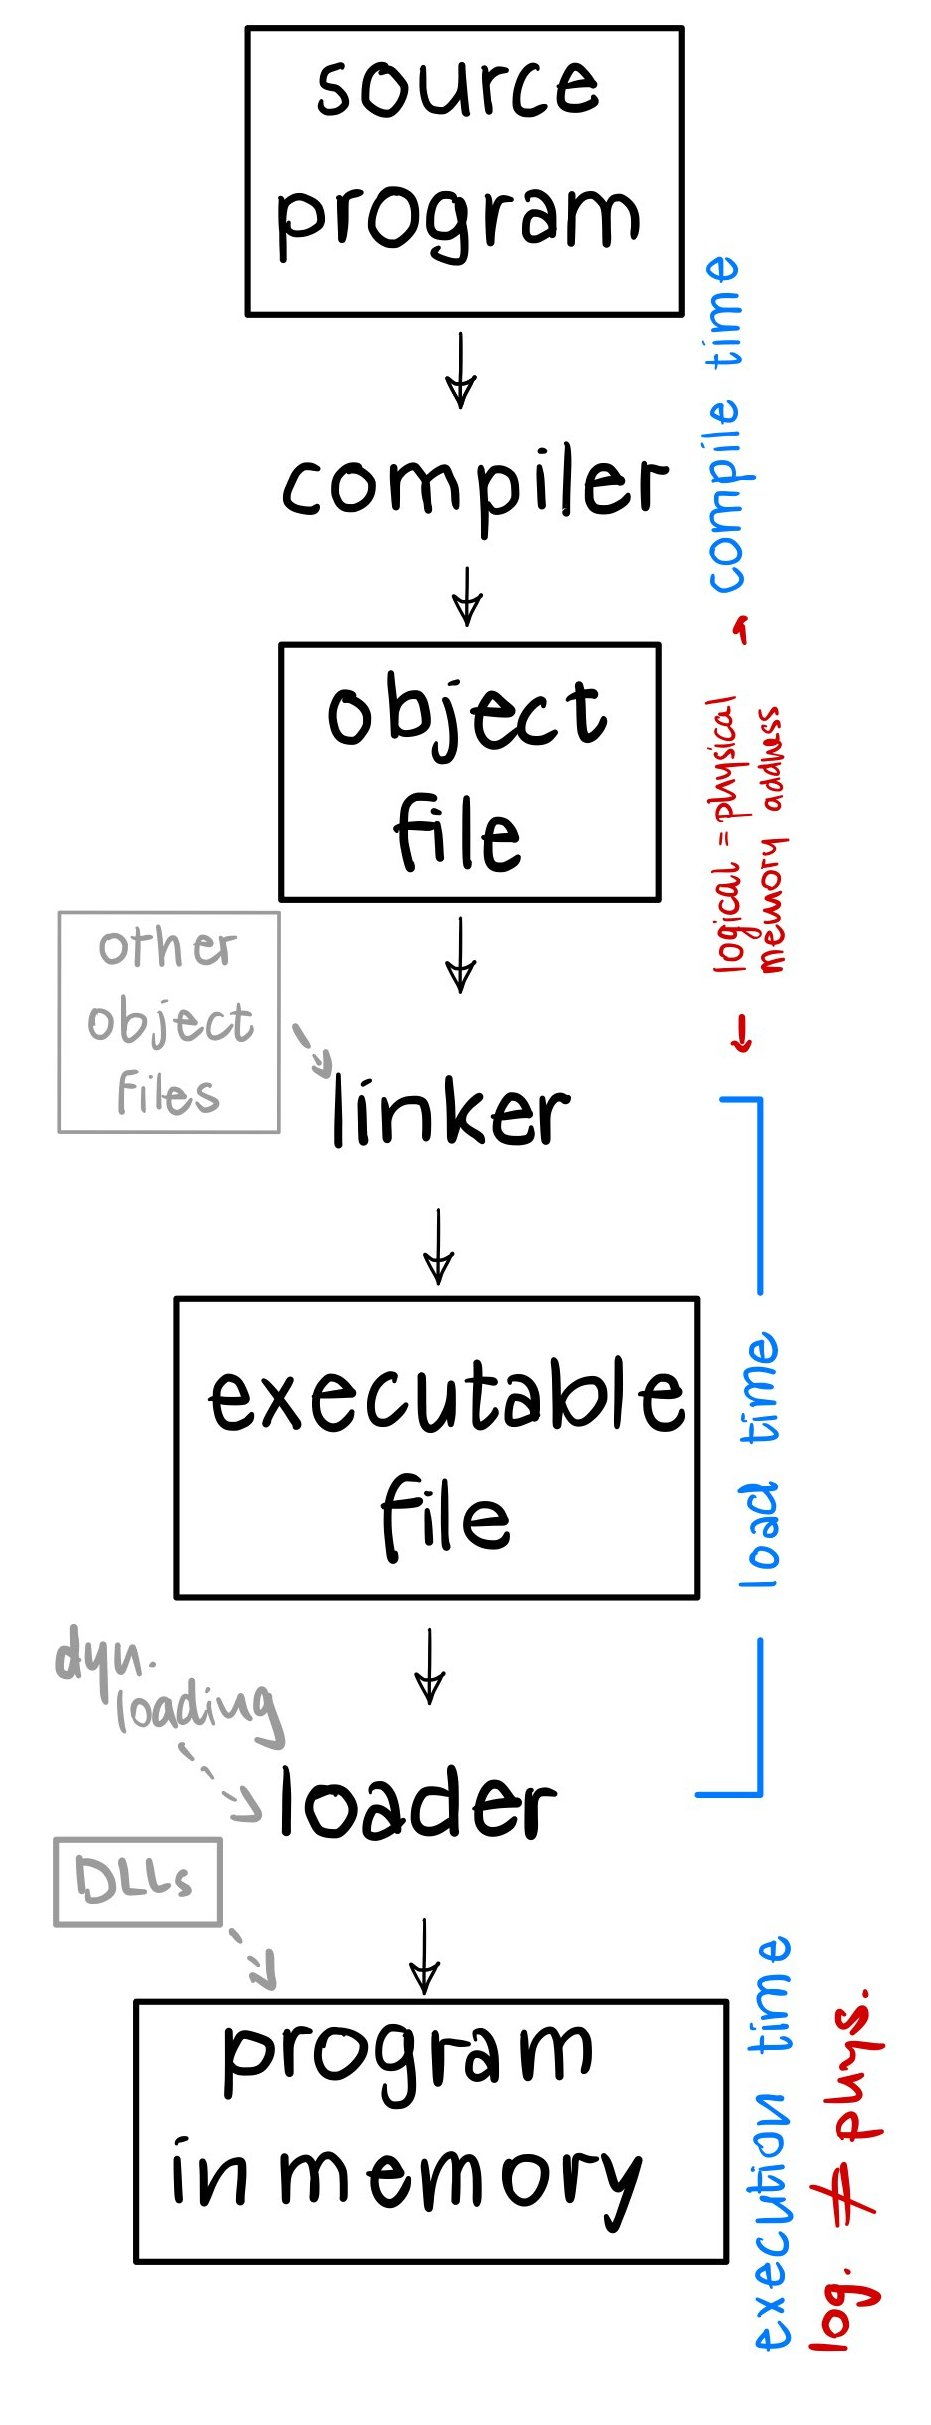
\includegraphics[width=15mm]{linking_loading.jpg}};
\end{tikzpicture}

\subsection*{Creation of processes}
\begin{description}
  \item[1. Preprocessing] Reads c file, processes \#include, expands macros, handles conditional compilation.
  \item[2. Compilation] Produces object code (.o), i.e. sequences of bytes, loadable into any mem location
  \item[3. Linking] Combines all object and library files into one executable file. Solves unresolved \\ external references. Relocates machine addresses
  \item[Dynamic Linking] Conditionally linked libraries. Loads system libraries only once.
  \item[Static Linking] Necessary library functions are embedded directly in exe.
  \item[4. Loading] Shell/click creates P, invokes loader, loads exe to RAM. OS allocates mem, \\ relocates mem addresses.
  \item[5. Execution] Program is a running P, CPU starts processing, upon completion returns status,\\ releases resources, removed from mem

  \item[Executables across OSs] Apps compiled on one OS are not executable on other OSs. \\ (differing system calls, binary formats, instruction sets application binary interface). Can be \\ solved via interpreted langs, virtual machines, use of standard API with compiler generating \\ binaries in OS specific language (e.g. POSIX)
\end{description}

\subsection*{OS Structures}
\begin{description}
    \item[Monolithic Systems]Includes everything between user prog and HW. \textbf{+} fast kernel comm., little overhead, easy interaction between OS modules, \textbf{-} difficult to change/maintain (complexity), single failure can cause system crash.
\begin{itemize}
    \item \textbf{Loadable Kernel Modules}: ex: device drivers, loaded when needed. OO-approach. more flexible (kernel can communicate directly). (Linux has this) \\
    \item \textbf{Layered Module Structure} OS divided into layers, each implements a service and communicates only to lower level layers (Layer 0: HW $\rightarrow$ N: UI).
\end{itemize}
    \item[Microkernel Systems] Everything in user mode, except scheduling, virt. mem. and basic IPC in kernel mode. + easy to extend, + reliability and security, + easier to port, - more performance overhead of kernel and user space communication. %NOTE: communication between user modules through message passing
      \item[Hybrid Systems] Combines microkernel and monolitic approach to address performance, security, usability needs. OS partially in kernel and user mode e.g. Linux
\end{description}
